
\begin{frame}{Bonnes pratiques dans le numérique}{Conseil 1/115}

\begin{block}{Éliminer les fonctionnalités non essentielles}

\textbf{Description} : 70\% des fonctionnalités non essentielles et 45\% jamais utilisées.
Niveau ergonomie, on augmente la simplicité.

\textbf{Méthodes} : maquettes, MoSCoW.


\begin{minipage}[b]{0.5\linewidth}  
\begin{figure}
    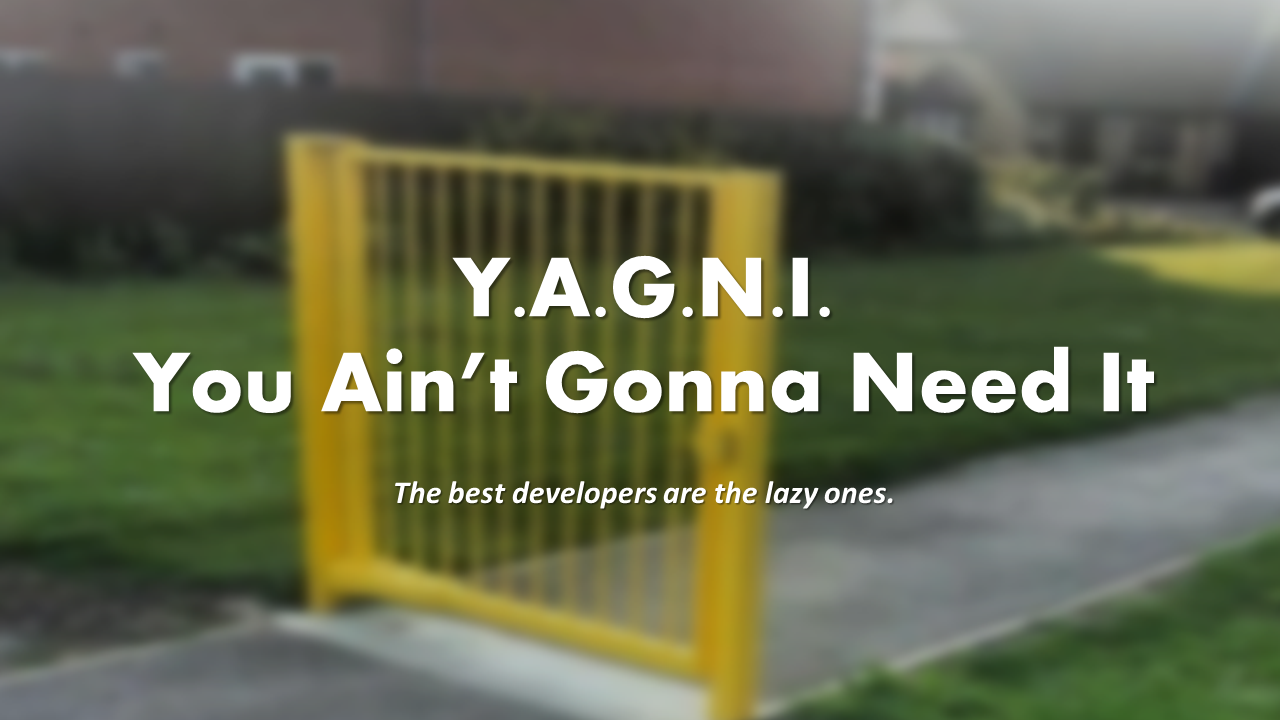
\includegraphics[scale=0.12]{chapitre2/wdd1/fig/yagni.png}
    \centering
\end{figure}
\end{minipage}\hfill
\begin{minipage}[b]{0.5\linewidth}  
\begin{figure}
    \centering
    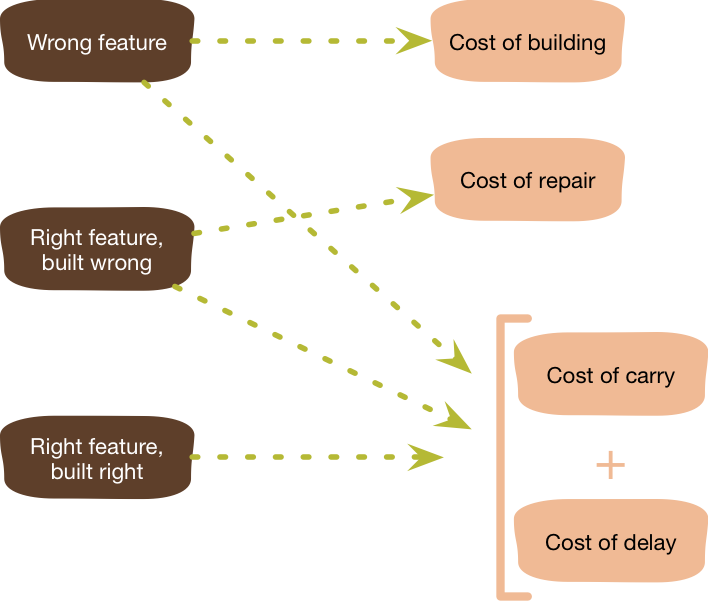
\includegraphics[scale=0.22]{chapitre2/wdd1/fig/sketch.png}
\end{figure}
\end{minipage}\hfill

\end{block}
\end{frame}

\begin{frame}{Bonnes pratiques dans le numérique}{Conseils 2-3/115}

\begin{block}{Quantifier précisément le besoin}

\textbf{Description} : Eviter la surqualité

\textbf{Exemples} : En l’absence de précision, le nombre d’items d’une liste est limité à 5 éléments.

Un nombre d’items affichés sur la page de résultats de son moteur de recherche Bing réduit jusqu’à 80\% le nombre de serveurs.

\end{block}

\begin{block}{Optimiser le parcours utilisateur}

\textbf{Description} : Diminuer le temps passé par l'utilisateur sur ses usages les plus fréquents

\textbf{Exemples} : 
\begin{enumerate}
    \item Proposer, pour un site de grande distribution, une nouvelle commande sur la base du contenu de la précédente
    \item Acheter sans inscription sur un site d'e-commerce.
    \item Copier/Coller son RIB plutôt que le télécharger puis le transférer.
    \item Mettre en avant les champs ou les filtres les plus utilisé
\end{enumerate}
\end{block}


\end{frame}

\begin{frame}{Bonnes pratiques dans le numérique}{Conseil 4/115}

\begin{block}{Préférer la saisie assistée à l'autocomplétion}

\textbf{Description} :L'autocomplétion envoie une requête au serveur à chaque caractère saisi pour récupérer les résultats correspondants (\textit{beaucoup de requêtes effectuées et de ressources dépensées}).

\textbf{Solution} :
Remplacer par la saisie assistée (guider l’utilisateur par un ensemble d’informations et d’indices)


\begin{figure}
    \centering
    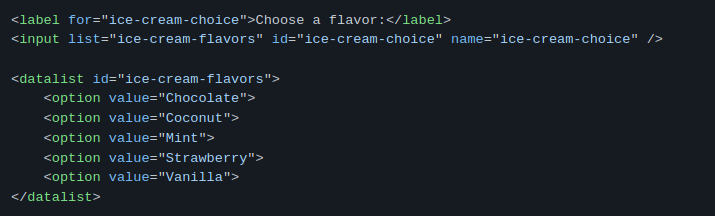
\includegraphics[scale=0.43]{chapitre2/wdd1/fig/codec.png}
\end{figure}


\end{block}

\end{frame}

\begin{frame}{Bonnes pratiques dans le numérique}{Conseils 5-6/115}

\begin{block}{Favoriser un design simple, épuré, adapté au web}

\textbf{Description} : Privilégier un design simple et épuré réalisable uniquement en HTML5 et CSS3.

\textbf{Méthode} :
 Supprimer les images de fond et ajouter un glyphe (Préférer les glyphes aux images, bonne pratique d'écoconception) avec une colorimétrie cohérente si un groupement doit avoir lieu.

\end{block}


\begin{block}{Privilégier une approche 'mobile first', à défaut un chargement adaptatif}

\textbf{Description} : Privilégier un design simple et épuré réalisable uniquement en HTML5 et CSS3.

\textbf{Exemples} :
\begin{enumerate}
    \item Côté serveur, utiliser les client hints,
    \item Côté client, media queries 
\end{enumerate}

\end{block}


\end{frame}



\begin{frame}{Bonnes pratiques dans le numérique}{Conseil 7/115}

\begin{block}{Respecter le principe de navigation rapide dans l’historique}

\textbf{Description} :
Eviter tout élément qui rendrait la page inéligible au bfcache, et/ou qui rendrait la page inutilisable après l'avoir quittée (\textit{ou éventuellement les rendre utilisables à nouveau quand la page est réutilisée, ou juste avant qu'elle soit mise en cache}).

\textbf{Solution : Eviter} 
\begin{enumerate}
    \item les actions lorsqu'on quitte la page (événements unload ou beforeunload, leur préférer pagehide si c'est vraiment nécessaire)
    \item les liens qui ouvrent de nouveaux onglets / fenêtres sans rel="noopener" ou rel="noreferrer"
    \item de laisser des connexions (IndexedDB, fetch() ou XMLHttpRequest, Web Sockets, etc.) ouvertes quand l'utilisateur quitte la page
\end{enumerate}

Utiliser les événéments \textbf{pageshow} et/ou \textbf{pagehide} pour réinitialiser les éléments, par exemple réactiver les boutons de formulaire qui se désactivent lors de la soumission ou supprimer les informations sensibles (\textit{comme les mots de passe}).
\end{block}

\end{frame}



\begin{frame}{Bonnes pratiques dans le numérique}{Conseil 8-9/115}

\begin{block}{Privilégier un traitement asynchrone}

\textbf{Description} :
Lorsque l’interaction avec l’utilisateur induit un traitement lourd et long côté serveur, proposer un traitement asynchrone.

\begin{itemize}
    \item Déclencher côté utilisateur le traitement
    \item se reconnecter quand celui-ci est terminé sans attendre sur son terminal la fin de l'exécution 
\end{itemize}


\textbf{Exemple} : Réception d’un e-mail contenant un lien. Cette approche permet de réaliser des traitements par lots (batchs), souvent plus efficients en ressources que des traitements synchrones à la volée.
\end{block}


\begin{block}{Limiter le nombre de requêtes HTTP}

\textbf{Description} :
Limiter le nombre de requêtes GET.


\textbf{Exemple} : Pour afficher des petits drapeaux pour le choix d'une langue, l'utilisation d'une spritesheet CSS permet de les regrouper dans une seule image de plus grande taille. Ce procédé réduit le nombre de requêtes HTTP.
\end{block}

\end{frame}



\begin{frame}{Bonnes pratiques dans le numérique}{Conseil 10/115}

\begin{block}{Stocker les données statiques localement}

\textbf{Description} :
Stocker localement des données structurées statiques (IndexDB, Web Storage et la mise en cache dans le Cache Storage API).

\end{block}

\begin{figure}
    \centering
    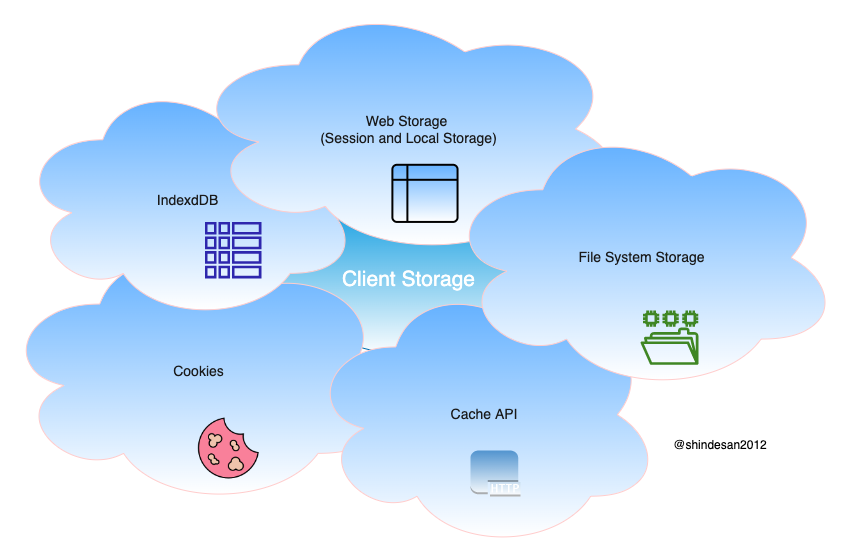
\includegraphics[scale=0.29]{chapitre2/wdd1/fig/storage.png}
\end{figure}

\end{frame}



\begin{frame}{Pause débunkage }{Fake checking : le véhicule électrique}

\begin{figure}
    \centering
    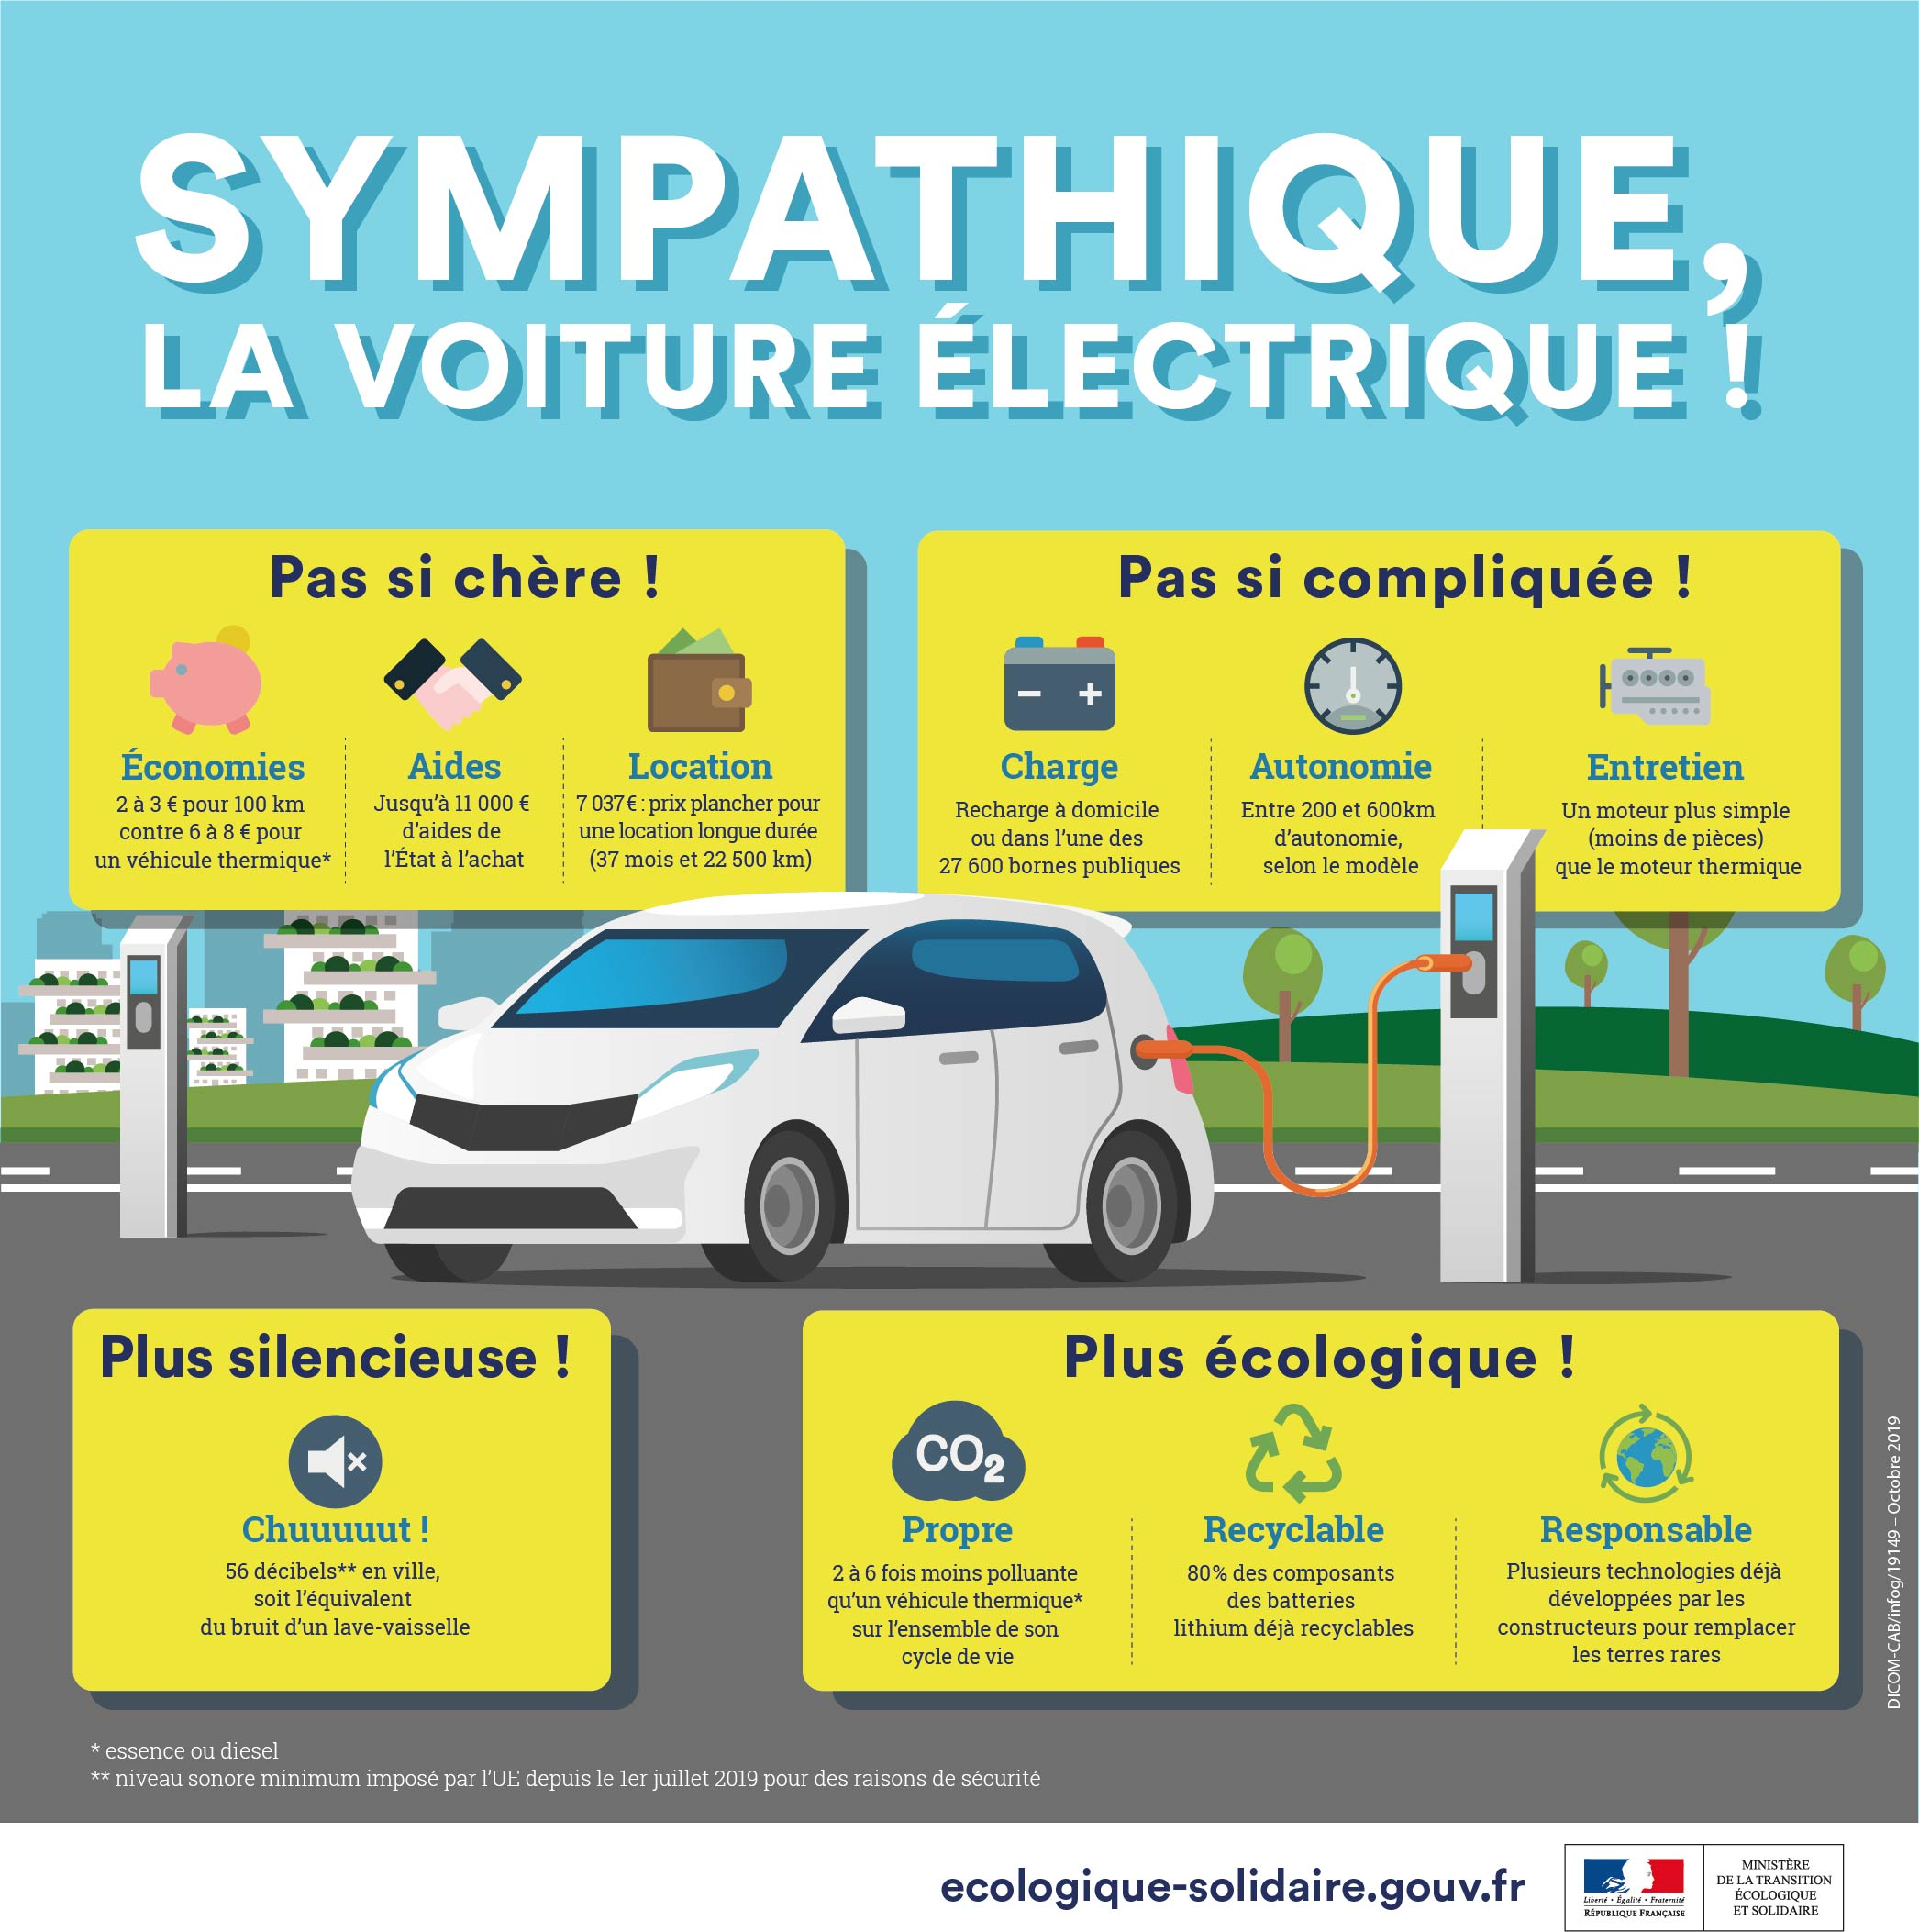
\includegraphics[scale=0.2]{chapitre2/wdd1/fig/ecovoiture.jpeg}
\end{figure}

%https://reporterre.net/Non-la-voiture-electrique-n-est-pas-ecologique#nb4

\end{frame}
